\documentclass[,man,floatsintext]{apa6}
\usepackage{lmodern}
\usepackage{amssymb,amsmath}
\usepackage{ifxetex,ifluatex}
\usepackage{fixltx2e} % provides \textsubscript
\ifnum 0\ifxetex 1\fi\ifluatex 1\fi=0 % if pdftex
  \usepackage[T1]{fontenc}
  \usepackage[utf8]{inputenc}
\else % if luatex or xelatex
  \ifxetex
    \usepackage{mathspec}
  \else
    \usepackage{fontspec}
  \fi
  \defaultfontfeatures{Ligatures=TeX,Scale=MatchLowercase}
\fi
% use upquote if available, for straight quotes in verbatim environments
\IfFileExists{upquote.sty}{\usepackage{upquote}}{}
% use microtype if available
\IfFileExists{microtype.sty}{%
\usepackage{microtype}
\UseMicrotypeSet[protrusion]{basicmath} % disable protrusion for tt fonts
}{}
\usepackage{hyperref}
\hypersetup{unicode=true,
            pdftitle={Simulation-Based Power-Analysis for Factorial ANOVA Designs},
            pdfauthor={Daniël Lakens~\& Aaron Caldwell},
            pdfkeywords={power analysis, ANOVA, hypothesis test, sample size justification},
            pdfborder={0 0 0},
            breaklinks=true}
\urlstyle{same}  % don't use monospace font for urls
\usepackage{graphicx,grffile}
\makeatletter
\def\maxwidth{\ifdim\Gin@nat@width>\linewidth\linewidth\else\Gin@nat@width\fi}
\def\maxheight{\ifdim\Gin@nat@height>\textheight\textheight\else\Gin@nat@height\fi}
\makeatother
% Scale images if necessary, so that they will not overflow the page
% margins by default, and it is still possible to overwrite the defaults
% using explicit options in \includegraphics[width, height, ...]{}
\setkeys{Gin}{width=\maxwidth,height=\maxheight,keepaspectratio}
\IfFileExists{parskip.sty}{%
\usepackage{parskip}
}{% else
\setlength{\parindent}{0pt}
\setlength{\parskip}{6pt plus 2pt minus 1pt}
}
\setlength{\emergencystretch}{3em}  % prevent overfull lines
\providecommand{\tightlist}{%
  \setlength{\itemsep}{0pt}\setlength{\parskip}{0pt}}
\setcounter{secnumdepth}{0}
% Redefines (sub)paragraphs to behave more like sections
\ifx\paragraph\undefined\else
\let\oldparagraph\paragraph
\renewcommand{\paragraph}[1]{\oldparagraph{#1}\mbox{}}
\fi
\ifx\subparagraph\undefined\else
\let\oldsubparagraph\subparagraph
\renewcommand{\subparagraph}[1]{\oldsubparagraph{#1}\mbox{}}
\fi

%%% Use protect on footnotes to avoid problems with footnotes in titles
\let\rmarkdownfootnote\footnote%
\def\footnote{\protect\rmarkdownfootnote}


  \title{Simulation-Based Power-Analysis for Factorial ANOVA Designs}
    \author{Daniël Lakens\textsuperscript{1}~\& Aaron Caldwell\textsuperscript{2}}
    \date{}
  
\shorttitle{ANOVA Power}
\affiliation{
\vspace{0.5cm}
\textsuperscript{1} Eindhoven University of Technology, The Netherlands\\\textsuperscript{2} Department of Health, Human Performance and Recreation, University of Arkansas, USA}
\keywords{power analysis, ANOVA, hypothesis test, sample size justification\newline\indent Word count: 5000}
\usepackage{csquotes}
\usepackage{upgreek}
\captionsetup{font=singlespacing,justification=justified}

\usepackage{longtable}
\usepackage{lscape}
\usepackage{multirow}
\usepackage{tabularx}
\usepackage[flushleft]{threeparttable}
\usepackage{threeparttablex}

\newenvironment{lltable}{\begin{landscape}\begin{center}\begin{ThreePartTable}}{\end{ThreePartTable}\end{center}\end{landscape}}

\makeatletter
\newcommand\LastLTentrywidth{1em}
\newlength\longtablewidth
\setlength{\longtablewidth}{1in}
\newcommand{\getlongtablewidth}{\begingroup \ifcsname LT@\roman{LT@tables}\endcsname \global\longtablewidth=0pt \renewcommand{\LT@entry}[2]{\global\advance\longtablewidth by ##2\relax\gdef\LastLTentrywidth{##2}}\@nameuse{LT@\roman{LT@tables}} \fi \endgroup}


\usepackage{lineno}

\linenumbers

\authornote{All code used to create this manuscript is
provided in an OSF repository at \url{https://osf.io/xxxxx/}.

Correspondence concerning this article should be addressed to Daniël
Lakens, ATLAS 9.402, 5600 MB, Eindhoven, The Netherlands. E-mail:
\href{mailto:D.Lakens@tue.nl}{\nolinkurl{D.Lakens@tue.nl}}}

\abstract{
Researchers need to design informative studies. When the goal of an
experiment is to test a hypothesis based on a frequentist hypothesis
test it is important to justify the sample size based on the statistical
power of the study. However, researchers are faced with challenges when
they try to calculate power for factorial ANOVA designs. First, current
software solutions are limited as they do not allow power analyses for
more complex designs involving multiple within factors. Second, they
require partial eta-squared or Cohen's f as input, which are not the
most intuitive way to specify predicted effects in an ANOVA, and do not
generalize to different experimental designs. We have created R
functions and an online Shiny app that performs simulations for ANOVA
designs for up to three factors with an unlimited number of levels.
Predicted effects are entered by specifying means, standard deviations,
and correlations (for within factors). The simulation provides a-priori
power analyses for all effects in the ANOVA, and all simple comparisons.
No other software is currently available that allows researchers to so
easily perform power analyses for a wide range of ANOVA designs. The app
plots \emph{p}-value distributions for all tests, and allows researchers
to select a range of options to correct for multiple comparisons. This
tutorial will teach researchers how to perform power analysis for ANOVA
designs, and through simulations illustrate important factors that
determine the statistical power of factorial ANOVA designs.


}

\begin{document}
\maketitle

Statistical power is the probability of observing a statistically
signficant result, given a specified effect size, and assuming there is
a true effect. When a researcher aims to analyze a study based on an
analysis of variance (ANOVA), the sample size of the study should be
justified based on the statistical power of the test. A study has low
power to detect effects the researcher is interested in has a high Type
2 error rate, and leads to a high probability of saying there is no
effect, when there actually is a true effect to be found. Whereas power
analyses for simple comparisons are relatively easy to perform, an
a-priori power analysis for factorial ANOVA designs is a challenge.
Available software solutions do not provide easy options for more
complex designs (e.g., a 2x2x2 design, where the first factor is
manipulated between participants, and the last two factors are
manipulated within participants). Popular software solutions such as
G*power require participants to enter their predictions as Cohen's f or
partial eta squared, which are not the most intuitive ways to specify a
hypothesized pattern of results, and which do not generalize to
different experimental designs.

Here, we demonstrate how to perform power analyses for factorial ANOVA
designs based on simulations. We provide R code and a Shiny app that can
be used to calculate the statistical power based on a predicted pattern
of means, standard deviations, and correlations (for within factors).
Simulating studies, and calculating their \emph{p}-values and effect
sizes, are a useful way to gain a better understanding of the factors
that determine the statistical power of hypothesis tests. After
providing an introduction to statistical power in general, and for the
\emph{F}-test specifically, we will demonstrate how the power of
factorial ANOVA designs depends on the pattern of means across
conditions, the number of factors and levels, and the sample size. We
will also illustrate the importance of controlling Type 1 error rates in
exploratory ANOVA's, and the importance to design studies that have high
power for main effects and interactions in an ANOVA, but also for
follow-up tests for simple effects.

\section{Factors That Determine Power in ANOVA
Designs}\label{factors-that-determine-power-in-anova-designs}

You perform a study in which participants interact with an artificial
voice assistant who sounds either cheerful or sad. You measure how much
70 participants in each condition enjoy interacting with the voice
assistant on a line marking scale (coded continously from -5 to 5) and
observe a mean of 0 in the sad condition, and a means of 1 in the
cheerful condition, with an estimated standard deviation of 2. After
submitting your manuscript for publications, reviewers ask you to add a
study with a neutral control condition to examine whether cheerful
voices increase, or sad voices decrease enjoyment (or both). Depending
on what the mean in the neutral condition is, which sample size would
you need to have a high powered study for the expected pattern or means?
A collaborator suggests to switch from a between design to a within
design, to more efficiently collect the data. Which consequence will
this switching to a within-subject design have on the sample size
planning? Because the effect size in the first study could be considered
\enquote{medium} based on the benchmarks by Cohen (1988), does it make
sense to plan for a \enquote{medium} effect size in either the between
of within ANOVA design? And if you justify the sample size based on the
ANOVA, will the study also have sufficient statistical power for the
simple effects (or vice versa)?

Performing simulation studies is an excellent way to develop intuitions
about these questions. The power in ANOVA designs depends on the pattern
of means, the number of groups, the standard deviation, the correlation
between dependent measures, the alpha level, and the sample size. After
these factors have been specified, a simulation study can be perform to
run the planned statistical test on generated data many times, and
summarize the results. Where analytic power solutions exists in software
such as G*Power for ANOVA designs with up to one within-subject factor,
simulation studies are more flexible (and can for example be used to see
what happens in a 3x3x3 within-subject desing).

\section{Statistical Power When Comparing Differences Among Group
Means}\label{statistical-power-when-comparing-differences-among-group-means}

Let's consider the initial study we described above, where two group
means are compared. We can test the difference between two means with a
\emph{t}-test of a one-way single factor ANOVA, and the two tests are
mathematically equivalent. Figure \ref{fig:d-plot} and Figure
\ref{fig:eta-plot} visualize the distribution of Cohen's d and partial
eta-squared that should be observed when there is no effect (grey
curves) and when the observed difference between means equals the true
effect. In both figures the light grey areas under the curve mark the
observed results that would lead to a Type 1 error (observing a
statistically significant result if the null-hypothesis is true) and the
dark grey areas under the curve marks the observed effect sizes that
would lead to a Type 2 error. An observed effect is statistically
significant if the observed effect size is larger than the critical
value. Critical values are often expressed as \emph{t}-values or
\emph{F}-values, but can be expressed as effect sizes (Cohen's d and
partial eta-squared), and any observed effect size larger than the
critical effect size will be statistically significant. The goal of
power analysis is to choose a sample size so that the probability of
observing a statistically significant effect for a specified effect size
reaches a desired probability. In both Figures, 83.5\% of the expected
effect sizes, if the true effect size is d = 0.5 or \(\eta_p^2\) =
0.0588 and 70 participants in each condition are collected, will be more
extreme than the critical effect size (which is d = 0.334 or
\(\eta_p^2\) = 0.028).

\begin{figure}
\centering
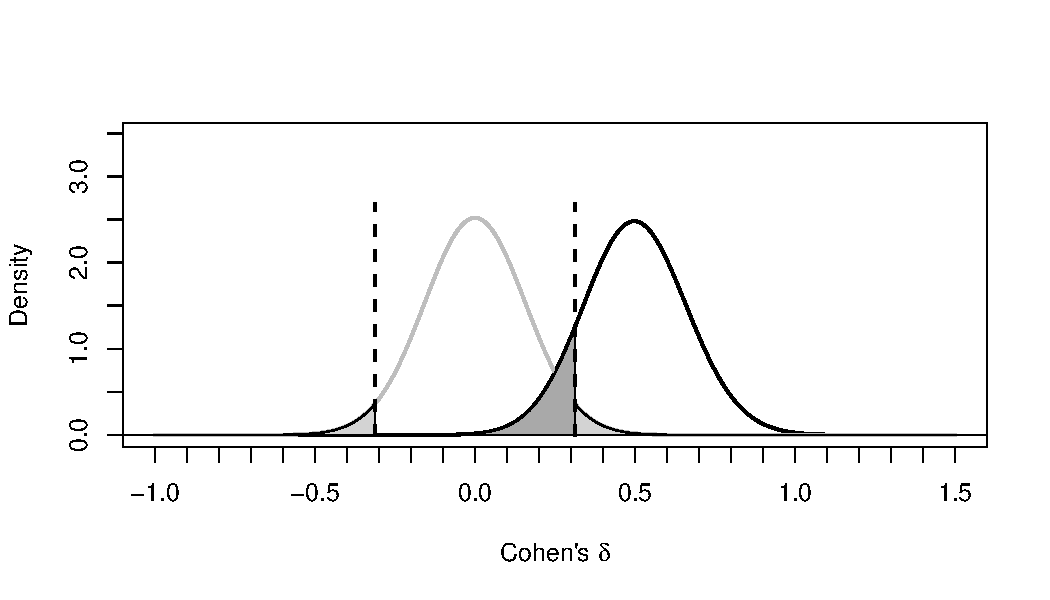
\includegraphics{0.1_Simulation_Based_Power_Analysis_For_Factorial_ANOVA_Designs_files/figure-latex/d-plot-1.pdf}
\caption{\label{fig:d-plot}Distribution of Cohen's d under the
null-hypothesis (grey curve) and alternative hypothesis assuming d = 0.5
(black curve). Note that}
\end{figure}

\begin{figure}
\centering
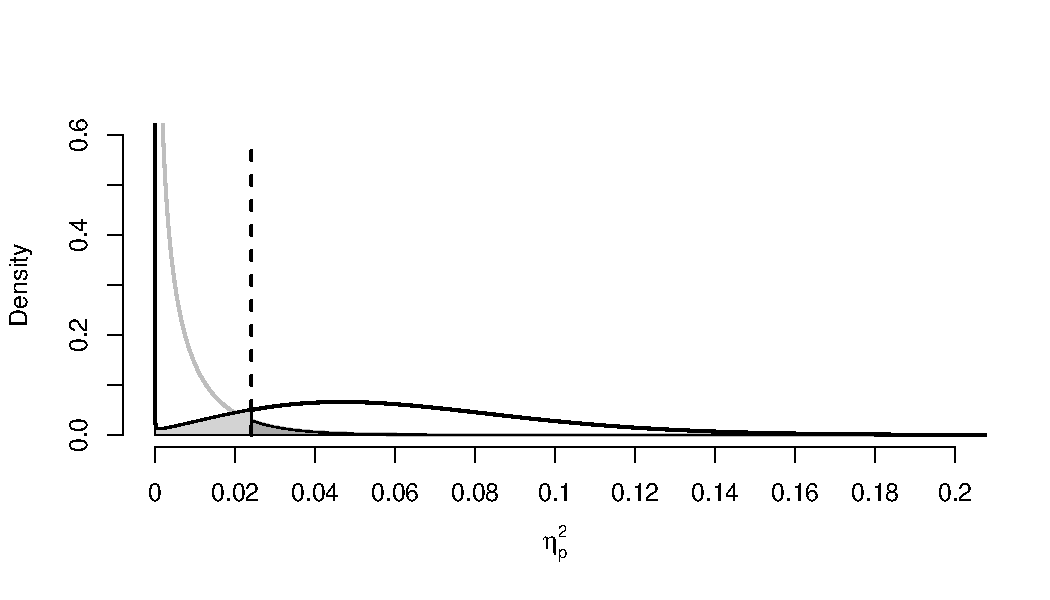
\includegraphics{0.1_Simulation_Based_Power_Analysis_For_Factorial_ANOVA_Designs_files/figure-latex/eta-plot-1.pdf}
\caption{\label{fig:eta-plot}Distribution of eta-squared under the
null-hypothesis (grey curve) and alternative hypothesis assuming partial
eta-squared = 0.0588 (black curve).}
\end{figure}

Two relationships between the \emph{t}-test and the \emph{F}-test when
comparing two means are worth pointing out. First, \(F = t^2\), or the
\emph{F}-value equals the \emph{t}-value, squared. Whereas we typically
think of a \emph{t}-test as the difference between means, the
relationship between the \emph{t}-test and \emph{F}-test reveals that we
can also use the group means to calculate the variance of the difference
between the two means \((m_1 - m_2)^2\). The \emph{F}-test is used to
compute the ratio of the between group variance and the within group
variance, and the between group variance can be used to compare more
than two means. The second relationship between a \emph{t}-test and a
\emph{F}-test for two groups is that the effect size for an ANOVA,
Cohen's f, is half the size of the effect size for standardized mean
differences, Cohen's d, of \(f = \frac{1}{2}d\). Cohen's d is calculated
by dividing the difference between means by the standard deviation, or

\begin{equation}
d = \frac{m_1-m_2}{\sigma}.
\end{equation}

If we have two groups with means of 1 and 2, and the standard deviation
is 2, Cohen's d is (2-1)/2, or 0.5. Cohen's f is the standard deviation
of the population means divided by the population standard deviation
(Cohen, 1988), or:

\begin{equation}
f = \frac{\sigma _{ m }}{\sigma}
\end{equation}

where for equal sample sizes,

\begin{equation}
\sigma _{ m } = \sqrt { \frac { \sum_ { i = 1 } ^ { k } ( m _ { i } - m ) ^ { 2 } } { k } }.
\end{equation}

Because Cohen's f is an essential part of power power analyses for
factorial ANOVA designs, it is worth illustrating how it is calculated
in an example. If we again take two means of 1 and 2, and a standard
deviation of 2, the grand mean is 1.5. We subtract each condition mean
from the grand mean, take the square, calculate the sum of squares,
divide it by two, and take the square root.
\(\sigma_m = \sqrt{\frac{(1-1.5)^2+(2-1.5)^2}{2}} = \sqrt{\frac{0.25+0.25}{2}} = 0.5\),
and \(f = \frac{0.5}{2} = 0.25.\) We see Cohen's f is half as large as
Cohen's d. Power analyses for ANOVA are based on Cohen's f, but popular
power anaysis software such as G*Power (Faul, Erdfelder, Lang, \&
Buchner, 2007) also allows researchers to specify the effect size as
partial eta-squared (\(\eta_p^2\)). Partial eta-squared can be converted
into Cohen's f:

\begin{equation}
f = \sqrt{\frac{\eta_p^2}{1-\eta_p^2}}
\end{equation}

and Cohen's f can be converted into partial eta-squared:

\begin{equation}
\eta_p^2 = \sqrt{\frac{f^2}{f^2+1}}
\end{equation}

In the example above, \(\eta_p^2 = 0.25^2/(0.25^2+1) = 0.0588\).

Because Cohen's f is calculated based on the sum of squares, the value
is always positive, just as the \emph{F}-value for an ANOVA is always
positive.

\newpage

\section{References}\label{references}

\setlength{\parindent}{-0.5in} \setlength{\leftskip}{0.5in}

\hypertarget{refs}{}
\hypertarget{ref-cohen_statistical_1988}{}
Cohen, J. (1988). \emph{Statistical power analysis for the behavioral
sciences} (2nd ed.). Hillsdale, N.J: L. Erlbaum Associates.

\hypertarget{ref-faul_gpower_2007}{}
Faul, F., Erdfelder, E., Lang, A.-G., \& Buchner, A. (2007). GPower 3: A
flexible statistical power analysis program for the social, behavioral,
and biomedical sciences. \emph{Behavior Research Methods}, \emph{39}(2),
175--191.
doi:\href{https://doi.org/10.3758/BF03193146}{10.3758/BF03193146}


\end{document}
